\documentclass{zc-ust-hw}

\usepackage[]{lipsum} 

\name{SalahDin Ahmed Salh Rezk}
\id{202201079}
\course{Thermodynamics, Wave Motion and Optics}
\assignment{Assignment 7}

\usepackage{import}
\usepackage{xifthen}
\usepackage{pdfpages}

\newcommand{\incfig}[1]{%
    \def\svgwidth{\columnwidth}
    \import{./figures/}{#1.pdf_tex}
}

\newcommand{\midlabelline}[3]{
   \node (midlabel) at ($ (#1)!.5!(#2) $) {#3};
   \draw[<-] (#1) --  (midlabel);
   \draw[->] (midlabel) -- (#2);
}
%% Point
\newcommand{\point}[3]{
\draw[fill=black] (#1) circle (1pt) node[#3] {#2};
}

\usepackage{tikz}

\tikzset{>=latex}
\usetikzlibrary{decorations.markings, calc}

\begin{document}

\maketitle

\begin{enumerate}
  \item For each of the cases below, identify all modes of heat transfer
    (conduction, convection, or radiation) that contribute to the cooling or
    heating, and describe each. Clearly state the object(s) involved in each
    mode and the direction of heat transfer. 
    \begin{enumerate}
      \item A slice of bread is heated in a toaster. 
        \begin{sol}
          To toast a slice of bread in a toaster, various heat transfer
          mechanisms come into play. Firstly, the heating element in the
          toaster transfers heat to the surrounding air through both convection
          and radiation. Subsequently, the heated air around the coil conveys
          heat to the bread via convection. There is a possibility of heat loss
          through convection if the air inside the toaster has not warmed up
          yet. Additionally, the heating element directly transfers heat to the
          toast through convection, especially in pop-up toasters where there
          is direct contact between the heating wire and the bread, allowing
          heat to travel through conduction.
        \end{sol}
      \item A kettle is filled with cold water and is heated on an electric stovetop until the water boils. 
        \begin{sol}
          When heating a kettle filled with cold water on an electric stovetop
          until it reaches boiling point, heat is transferred through a
          combination of conduction and radiation. Initially, the stove's
          heating element transfers heat directly to the bottom of the kettle.
          The heat then travels through the kettle's bottom surface by
          conduction and is further conveyed to the water by convection. Some
          heat is lost to the kettle's side walls and top through convection,
          and the top and sides transfer heat through conduction. Throughout
          the process, there is convection all around the kettle, leading to
          potential heat gain or loss on the bottom side.
        \end{sol}
      \item A can of soda is placed in a refrigerator to cool. 
        \begin{sol}
          Cooling a can of soda in a refrigerator involves heat transfer
          mechanisms. Heat from the soda moves to the can's wall through
          convection. Subsequently, the heat travels through the can via
          conduction, eventually transferring to the refrigerator air through
          convection. Heat loss occurs through the can's bottom due to
          conduction, especially where the can is in contact with the fridge
          rack.
        \end{sol}
      \item Cake batter is poured into a cake pan, which is placed into an oven to bake. 
        \begin{sol}
          Baking cake batter in an oven involves a complex interplay of heat
          transfer methods. The oven's heating element initially transfers heat
          to the air through convection. The heated air then conveys heat to
          the cake pan and the top surface of the cake via convection. Heat
          travels through the cake pan by conduction. The cake batter receives
          heat from the oven air and the hot pan through either conduction or
          convection, depending on whether the batter is considered solid or
          fluid. Additionally, some heat is radiated from the oven heating
          element to the pan.
        \end{sol}
    \end{enumerate}
  \item When the thermal conductivity of a medium varies linearly with
    temperature, is the average thermal conductivity always equivalent to the
    conductivity value at the average temperature? 
    \begin{sol}
      \begin{align}
        \bar{k}&=\frac{1}{T_2-T_1} \int_{T_1}^{T_2} k d T \\
               &=\frac{1}{T_2-T_1} \int_{T_1}^{T_2}(a+b T) d T\\
               &=\frac{a\left(T_2-T_1\right)+b\left(T_2^2-T_1^2\right) / 2}{T_2-T_1}\\
               &=a+b \frac{T_2+T_1}{2}
      \end{align}
      If the thermal conductivity varies linearly with temperature, then the
      average thermal conductivity will always be the same as the thermal
      conductivity at the average temperature.
    \end{sol}

  \item  A steel ball bearing is 4.00 cm in diameter at 20.0\textdegree C. A brass plate
    has a hole in it that is 3.994 cm in diameter at 20.0\textdegree C. What common
    temperature must they have so that the ball just squeezes through the hole?
    Thermal expansion coefficients of steel and brass are \(1.2\times 10^{-5}\text{ C}^{-1}\)
    and \(2\times 10^{-5}\text{ C}^{-1}\) respectively.
    \begin{figure}[H]
      \begin{center}
        \includegraphics[width=0.95\textwidth]{figures/1705971983.png}
      \end{center}
      \caption{}\label{fig:}
    \end{figure}
    
    \begin{sol}
        \begin{gather}
          \left.4 \times\left[1+1.2 \times 10^{-5}(20-T)\right]=3.994 \times\left[1+2 \times 10^{-5}(20-T)\right]\right] \\
          1-\frac{3.994}{4}=(20-T)\left[\frac{3.994 \times 2 \times 10^{-5}}{4}-1.2 \times 10^{-5}\right] \\
          20-T=188.2^0 \mathrm{C} \\
          T=-168.2{ }^0 \mathrm{C}
        \end{gather}
    \end{sol}

  \item Estimate the percent change in density of iron when it is still a
    solid, but deep in the earth where the temperature is 2000\textdegree C and it is
    under 5000 atm of pressure. Take into account both thermal expansion and
    change due to increased outside pressure. Assume both the bulk modulus and
    the volume coefficient of expansion do not vary with temperature and are
    the same as at normal room temperature of 20\textdegree C. The bulk modulus for iron
    is about \(90\times 10^{9}\text{ N/m}^2\) and the coefficient of volume expansion \(35\times 10^{-6}\text{ C}^{-1}\).   
    \begin{sol}
      \begin{gather}
        \rho=\frac{m}{V} \quad \rightarrow \quad \frac{d \rho}{d V}=-\frac{m}{V^2}=-\frac{m}{V} \frac{1}{V} \\
        \frac{d \rho}{d V}=-\frac{\rho}{V} \quad \rightarrow \quad \frac{d \rho}{\rho}=-\frac{d V}{V} \\
        B=-\frac{\Delta P}{\Delta V / V} \quad \rightarrow \quad \frac{\Delta V}{V}=-\frac{\Delta P}{B} \\
        \Delta P=5000-1=4999 \mathrm{~atm}=4999 \times 1.01 \times 10^5 \mathrm{~Pa}=5.049 \times 10^8 \mathrm{~Pa} \\
        \frac{\Delta V}{V}=-\frac{5.049 \times 10^8}{90 \times 10^9}=-5.6 \times 10^{-3} \\
        \Delta V=V \beta \Delta T \\
        \Delta T=2000-20=1980^{\circ} \mathrm{C} \\
        \frac{\Delta V}{V}=\beta \Delta T=35 \times 10^{-6} \times 1980=6.93 \times 10^{-2} \\
        \text { Total } \frac{\Delta V}{V}=6.93 \times 10^{-2}-5.6 \times 10^{-3}=6.37 \times 10^{-2} \\
        \frac{d \rho}{\rho}=-\frac{\Delta V}{V}=-6.37 \times 10^{-2} \\
        \text { Or } \quad \frac{d \rho}{\rho}=-6.37 \%
      .\end{gather}
    \end{sol}

  \item A study shows that pet lizard makes a weird groaning noise every couple
    of seconds. they noticed that the number of groans per minute is very
    regular, but somehow increases as the temperature increases. Further
    observations reveal that the number of groans per minute actually has a
    linear relationship with temperature over the normal range of temperatures
    in the lizard's natural environment. So it is more like the lizard acts
    like a living thermometer. They measured that the number of groans per
    minute at 20.0°C is 30.0, and the number of groans per minute at 55.0 °C is
    35.2. If they measured that the number of groans per minute in the lizard's
    usual aquarium is 31.5, what is the temperature in the aquarium, in degrees
    Celsius?

    \begin{sol}
      \begin{align}
        \Delta G&=m\Delta T \\
        m&= \frac{\Delta G}{\Delta T} = \frac{5.2}{35} \\
         &= 0.15 \text{ C}^{-1} \\
        G(T)-G(20)&=m(T-20) \\
        1.5&=0.15(T-20) \\
        T&=30\text{\textdegree C}
      .\end{align}
    \end{sol}

  \item At very low temperature, the molar specific heat of many substances
    varies as the cube of the absolute temperature: 
    \[
      C=k \frac{T^3}{T_{0}^3}
    .\] 
    Which is sometimes called Debye’s law. For rock salt, \( T_{0} \) = 281 K and k =
    1940 J/mol. K. Determine the heat needed to raise 3.5 mol of salt from 22.0
    K to 55.0 K.  
    \begin{sol}
      \begin{align}
        dQ &= nCdT \\
        &= nk \frac{T^3}{T_{0}^3}dT \\
        Q &= \frac{nk}{T_{0}^3 }\int_{T_{1}}^{T_{2}}T^3 \,dT  \\
        &=\left.\frac{n k}{T_o^3} \frac{T^4}{4}\right|_{T_1} ^{T_2} \\
        &=\frac{n k}{4 T_o^3}\left[T_2^4-T_1^4\right] \\
        &=\frac{3.5 \times 1940}{4 \times 281^3}\left[55^4-22^4\right] \\
        &=682.1 \mathrm{~J}
      .\end{align}
    \end{sol}

    \newpage
    
  \item After baking a cake in the oven, you set the cake on a rack to cool.
    The cake is 8 cm high, and has a 20 cm diameter. I f the surface
    temperature of the cake is 90 °C on all sides and the air temperature in
    the room is 22 °C, calculate the rate of heat loss from the cake to the
    air. You may also find the following hints useful.
    \begin{enumerate}
      \item The convection coefficient can be approximated as 15 W/ m² K on the
        top and the side surfaces, and 5 W/m² K on the bottom surface. 
      \item The emissivity of the cake surface is 0.4 on all sides. 
      \item You may neglect the effects of heat loss due to conduction. 
    \end{enumerate}
    
    \begin{sol}
      \begin{equation}
      q_{\text {lost }}=q_{\text {convection,top }}+q_{\text {convection, top }}+q_{\text {convection, bottom }}+q_{\text {radiation, all sides }}
      \end{equation}
      \begin{align}
        q_{\text {convection,top }} & =h_{\text {top }} A_{\text {top }}\left(T-T_{\infty}\right) \\
        q_{\text {convection,bottom }} & =h_{\text {bottom }} A_{\text {bottom }}\left(T-T_{\infty}\right) \\
        q_{\text {convection, side }} & =h_{\text {side }} A_{\text {side }}\left(T-T_{\infty}\right) \\
        q_{\text {radiation, all sides }} & =\varepsilon \sigma A_{\text {total }} T^4
      \end{align}
      \begin{align}
        A_{\text {top }} & =A_{\text {bottom }}=\pi r^2=\pi(0.1)^2=0.03142 \mathrm{~m}^2 \\
        A_{\text {side }} & =2 \pi \mathrm{rh}=2 \pi(0.1)(0.08)=0.05027 \mathrm{~m}^2 \\
        A_{\text {total }} & =2 A_{\text {top }}+A_{\text {side }}=0.1131 \mathrm{~m}^2
      \end{align}
      \begin{align}
        q_{\text {convection,bottom }} & =h_{\text {bottom }} A_{\text {bottom }}\left(T-T_{\infty}\right)=5(0.03142)(90-22)=10.683 \\
        q_{\text {convection, side }} & =h_{\text {side }} A_{\text {side }}\left(T-T_{\infty}\right)=15(0.05027)(90-22)=51.271 \\
        q_{\text {radiation,all sides }} & =\varepsilon \sigma A_{\text {total }} T^4=0.4\left(5.67 \times 10^{-8}\right)(0.1131)(90+273)^4=44.54
      \end{align}

      \begin{align}
        q_{\text {lost }} & =q_{\text {convection, top }}+q_{\text {convection, top }}+q_{\text {convection, bottom }}+q_{\text {radiation, all sides }} \\
                          & =32.048+10.683+51.271+44.54 \\
                          & =138.5 \mathrm{~W}
      .\end{align}
    \end{sol}

    \newpage

  \item A platinum resistance thermometer is a device that allows us to
    determine the temperature by measuring the resistance of a piece of pure
    platinum wire. In the interval between the freezing point of water and
    700.0°C, the relationship between the resistance and the Celsius
    temperature $T_C$ is accurately captured by the formula $R = R_0 (1 + A T_C + B
    T_C^2 )$ where A and B are constants determined by measurements at the
    freezing point of water, the boiling point of water, and the melting point
    of lead (327.46°C).  

    \begin{enumerate}
      \item If R equals 5.000 ohms at the freezing point of water, 6.973 ohms
        at the boiling point of water,  and 10.80 ohms at the melting point of
        lead, find $R_0$, $A$, and $B$  
        \begin{sol}
          \begin{align}
            6.973 &= 5.000 (1+A\cdot 100+B\cdot 100^2) \\
            10.800 &= 5.000 (1+A\cdot 327.46+B\cdot 327.46^2) \\
                   &\downarrow \nonumber \\
            A &= 0.004123 \\
            B &= -1.776 \times 10^{-6} 
          .\end{align}
        \end{sol}
      \item If the resistance is measured to be 8.300 ohms, what is the
        temperature?  
        \begin{sol}
          \begin{align}
            8.3 &= 5(1+AT+BT^2) \\
                &\downarrow \nonumber \\
            T &= -\frac{A}{2B} \pm \frac{1}{2B} \sqrt{A^2 + 4B \cdot 0.74} \\
            &= 172.9
          .\end{align}
        \end{sol}
      \item Plot $R$ versus $T_C$ in the range from 0°C to 700.0°C. 
        \begin{figure}[H]
          \begin{center}
            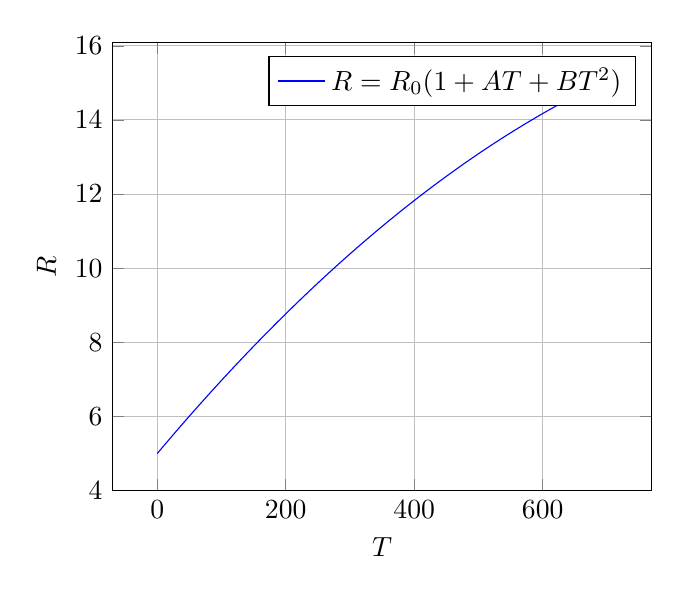
\begin{tikzpicture}
              \begin{axis}[
                xlabel={$T$},
                ylabel={$R$},
                legend pos=north east,
                grid=both,
                samples=100
                ]

                \def\Rzero{5}
                \def\A{0.004123}
                \def\B{-1.776e-6}

                \addplot[blue, domain=0:700, smooth] {\Rzero*(1 + \A*x + \B*x^2)};
                \legend{$R = R_0(1 + AT + BT^2)$}

              \end{axis}
            \end{tikzpicture}
          \end{center}
          \caption{}\label{fig:}
        \end{figure}
        
    \end{enumerate}

\end{enumerate}

\end{document}
